\documentclass[11pt]{article}
\usepackage{amsmath}
 \usepackage{amsfonts}
 \usepackage{amsthm}
 \usepackage{graphicx}   % need for figures
 \usepackage{verbatim}   % useful for program listings
 
 % Useful macros 
 \def\tcb#1{\color{blue}{#1}}
 \def\tcr#1{\color{red}{#1}}	
 \def\tcg#1{\color{green}{#1}}
 \def\be{\begin{eqnarray}}	 	\def\ee{\end{eqnarray}}
 \def\bea{\begin{eqnarray}}	 	\def\eea{\end{eqnarray}}
 \def\bean{\begin{eqnarray*}}	\def\eean{\end{eqnarray*}}
 
 \def\D{\displaystyle}
 \def\T{\textstyle}
 \def\l{\left}
 \def\r{\right}
 \def\nf{n_{\!f}} % quark flavours
 \def\pa{\partial}
 \def\eg{e.\,g.}
 \def\ie{i.\,e.}

 \def\be{\begin{equation}}
 \def\ee{\end{equation}}
 \def\bea{\begin{eqnarray}}
 \def\eea{\end{eqnarray}}
 \def\bean{\begin{eqnarray*}}
 \def\eean{\end{eqnarray*}}
 \def\gsim{\mathrel{\rlap{\lower0.2em\hbox{$\sim$}}\raise0.2em\hbox{$>$}}}
 \def\ksim{\mathrel{\rlap{\lower0.2em\hbox{$\sim$}}\raise0.2em\hbox{$<$}}}
 \def\kg{\mathrel{\rlap{\lower0.25em\hbox{$>$}}\raise0.25em\hbox{$<$}}}
 
 \def\AA{${\buildrel_{\circ} \over {\mathrm{A}}}$}
 \def\bm#1{\mbox{\boldmath$#1$}}
 \newcommand{\eq}[1]{(\ref{#1})} 
 \def\pd{\partial}
 \def\d{\textrm{d}} 
 \def\T{\textstyle}
 \def\eg{e.\,g.}	% exempli gratia (for the sake of example)
 \def\ie{i.\,e.}	% id est (that is)


 % Page configuration:
 \topmargin -2.0cm
 \oddsidemargin -0.85cm
 \evensidemargin -0.85cm
 \textwidth 18cm
 \textheight 24cm
\title{\textbf{Intermediate Test 1 Solutions}}
\date{\today}
\begin{document}

\begin{center}
\textbf{Stellenbosch Camp December 2017 \\ Intermediate Test 1} \\
\textbf{Solutions}
\end{center}

\begin{enumerate}

%QUESTION 1

\item The number of words with at least one $a$ can be calculated by subtracting the number of words not containing an $a$ from the total number of words that can be made. Since letters may be repeated, the total number of words possible is given by $26^5$. Those not containing an $a$ number $25^5$. Thus there are $26^5-25^5$ words containing at least one $a$.

%QUESTION 2

\item Let us assume for contradiction that 3 does not divide $ab$. Then neither $a$ nor $b$ can be divisible by 3, and hence $a^2 \equiv_3 1$ and $b^2 \equiv_3 1$. But then $8a^2+1\equiv_3 0 \Rightarrow b^2\equiv_3 0 \Rightarrow b\equiv_3 0$. This contradicts our initial assumption and so it must in fact be the case that $3\mid ab$.

%QUESTION 3

\item \textit{Solution using AM-GM inequality} \\
By the Arithmetic Mean-Geometric Mean inequality,
\begin{equation*}
\frac{a^2}{bc}+\frac{b^2}{ac}+\frac{c^2}{ab} \geq 3\sqrt[3]{\frac{a^2b^2c^2}{a^2b^2c^2}} = 3\sqrt[3]{1}=3
\end{equation*}
Thus proving the inequality as required. \\ \\
\textit{Alternative solution using first principles} \\
Simplifying, the inequality becomes
\begin{eqnarray*}
\frac{a^2}{bc}+\frac{b^2}{ac}+\frac{c^2}{ab} & \geq & 3 \\
\Leftrightarrow a^3+b^3+c^3 & \geq & 3abc \\
\Leftrightarrow (a+b+c)(a^2+b^2+c^2-ab-bc-ac) & \geq & 0
\end{eqnarray*}

Now $a+b+c \geq 0$, since $a,b,c$ are positive real numbers. $a^2+b^2+c^2-ab-bc-ac \geq 0 \Leftrightarrow (a-b)^2 + (b-c)^2 + (c-a)^2 \geq 0$, which is true since squares are non-negative. Thus each bracket on the lefthand side is non-negative, hence the lefthand side is non-negative and the inequality is proved.
 
 % QUESTION 4
    \item \textit{EGMO 2013, Problem 1} \\
    Define $F$ so that $ABFD$ is a parallelogram. Then $E, A, C, F$ are collinear (as diagonals of a parallelogram bisect each other) and $BF = AD = BE$. Further, $A$ is the midpoint of $EF$, since $AF = 2AC$, and thus $AB$ is an altitude of the isosceles triangle $EBF$ with apex $B$. Therefore $AB \perp AC$.
    
    % GEOMETRY FIGURE
    \begin{figure}[h!]
        \centering
        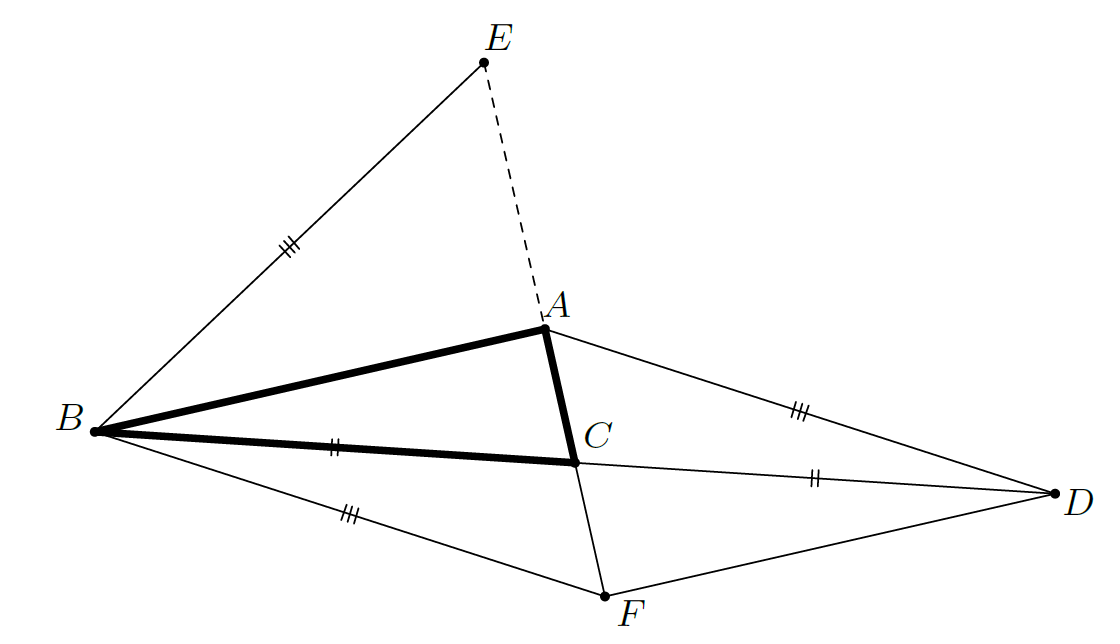
\includegraphics[width=0.4\textwidth]{seniortest1_q1.PNG}
    \end{figure}
    
    % QUESTION 2
    \item \textit{EGMO 2013, Problem 2} \\
    The solution naturally divides into three different parts: we first obtain some bounds on $m$. We then describe the structure of possible dissections, and finally, we deal with the few remaining cases.
    
    In the first part of the solution, we get rid of the cases with $m \leq 10$ or $m \geq 14$. Let $l_1, \dots, l_5$  and $w_1, \dots, w_5$ be the lengths and widths of the five rectangles. Then the rearrangement inequality yields the lower bound
    \begin{align*}
        l_1 w_1 &+ l_2 w_2 + l_3 w_3 + l_4 w_4 + l_5 w_5 \\
        &= \frac{1}{2} \left( l_1 w_1 + l_2 w_2 + l_3 w_3 + l_4 w_4 + l_5 w_5 + w_1 l_1 + w_2 l_2 + w_3 l_3 + w_4 l_4 + w_5 l_5 \right) \\
        &\geq \frac{1}{2} \left( 1 \cdot 10 + 2 \cdot 9 + 3 \cdot 8 + \dots + 8 \cdot 3 + 9 \cdot 2 + 10 \cdot 1 \right) = 110
    \end{align*}
and the upper bound
    \begin{align*}
        l_1 w_1 &+ l_2 w_2 + l_3 w_3 + l_4 w_4 + l_5 w_5 \\
        &= \frac{1}{2} \left( l_1 w_1 + l_2 w_2 + l_3 w_3 + l_4 w_4 + l_5 w_5 + w_1 l_1 + w_2 l_2 + w_3 l_3 + w_4 l_4 + w_5 l_5 \right) \\
        &\leq \frac{1}{2} \left( 1 \cdot 1 + 2 \cdot 2 + 3 \cdot 3 + \dots + 8 \cdot 8 + 9 \cdot 9 + 10 \cdot 10 \right) = 192.5
    \end{align*}


As the area of the square is sandwiched between $110$ and $192.5$, the only possible candidates for $m$ are $11$, $12$, and $13$.

In the second part of the solution, we show that a dissection of the square into five rectangles must consist of a single inner rectangle and four outer rectangles that each cover one of the four corners of the square. Indeed, if one of the sides the square had three rectangles adjacent to it, removing these three rectangles would leave a polygon with eight vertices, which is clearly not the union of two rectangles. Moreover, since $m > 10$, each side of the square has at least two adjacent rectangles. Hence each side of the square has precisely two adjacent rectangles, and thus the only way of partitioning the square into five rectangles is to have a single inner rectangle and four outer rectangles each covering the four corners of the square, as claimed.

Let us now show that a square of size $12 \times 12$ cannot be dissected in the desired way. Let $R_1, R_2, R_3$ and $R_4$ be the outer rectangles (in clockwise orientation along the boundary of the square). If an outer rectangle has a side of length $s$, then some adjacent outer rectangle must have a side of length $12 − s$. Therefore, neither of $s = 1$ or $s = 6$ can be sidelengths of an outer rectangle, so the inner rectangle must have dimensions $1 \times 6$. One of the outer rectangles (say $R_1$) must have dimensions $10 \times x$, and an adjacent rectangle (say $R_2$) must thus have dimensions $2 \times y$. Rectangle $R_3$ then has dimensions $(12 − y) \times z$, and rectangle $R_4$ has dimensions $(12 - z) \times (12 - x)$. Note that exactly one of the three numbers $x, y, z$ is even (and equals 4 or 8), while the other two numbers are odd. Now, the total area of all five rectangles is
$$ 144 = 6 + 10x + 2y + (12 - y) z + (12 - z)(12 - x), $$

which simplifies to $(y - x)(z - 2) = 6$. As exactly one of the three numbers $x, y, z$ is even, the factors $y - x$ and $z - 2$ are either both even or both odd, so their product cannot equal 6, and thus there is no solution with $m = 12$.

Finally, we handle the cases $m = 11$ and $m = 13$, which indeed are solutions. The corresponding rectangle sets are $10 \times 5, 1 \times 9, 8 \times 2, 7 \times 4$ and $3 \times 6$ for $m = 11$, and $10 \times 5, 9 \times 8, 4 \times 6, 3 \times 7$ and $1 \times 2$ for $m = 13$. These sets can be found by trial and error. The corresponding partitions are shown in the figure below.

    \begin{figure}[h!]
        \centering
        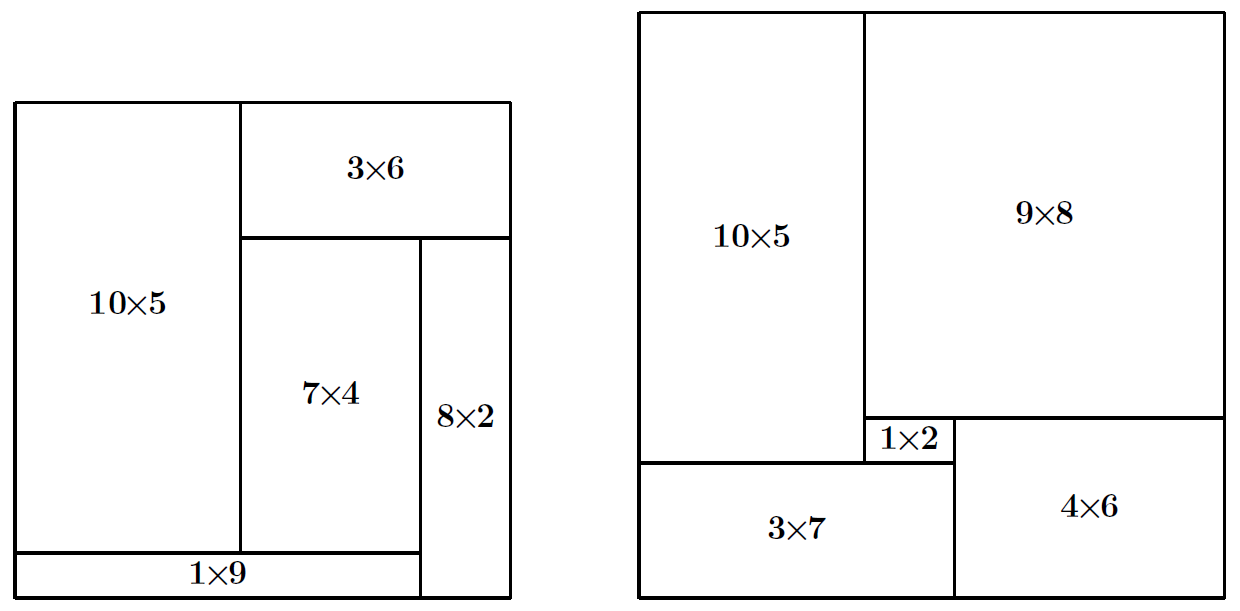
\includegraphics[width=0.8\textwidth]{seniortest1_q2.PNG}
    \end{figure}
    
    \textit{Remark:} The configurations for $m = 11$ and $m = 13$ given above are not unique.

\end{enumerate}

\end{document}
